\chapter{Estado del arte}\label{estadoarte}

Aquí se encuentra la parte teórica y tecnológica del proyecto. Se hablará de la identificación de tráfico y de 
las distintas técnicas que existen para ello. También se hablará de Bro \cite{broindex}, el 
analizador de tráfico que se usará para 
llevar a cabo el desarrollo del módulo. Se introducirá en que consiste, cómo gestiona los eventos y sus 
funcionalidades básicas, así como la posibilidad de ampliar estas.

\intro Por último se presentará de forma teórica en que consiste el emparejamiento de flujos y de qué forma 
se podría usar para identificar el tráfico.

\section{Identificación de tráfico}

Hay que tener claro que identificar el tráfico no es clasificarlo. Identificar el tráfico consiste en analizarlo 
y obtener patrones comunes con los cuales se pueda ordenar el tráfico de forma posterior. Algunos de los patrones 
que se pueden tener en cuenta a la hora de identificar tráfico son los puertos, las IP's o la clase a la que 
pertenece.

\intro Por lo tanto la identificación del tráfico de la red es esencial para realizar una clasificación 
posterior. Dicha clasificación se podrá analizar en busca de amenazas o intrusos, a nivel de seguridad 
y componentes lentos o defectuosos que afecten al rendimiento del servicio. Para poder identificar el 
tráfico lo deseable es un método que sea rápido y proteja la privacidad de los distintos usuarios.

\subsection{Técnicas de identificación de tráfico}

Existen varias técnicas de identificación de tráfico, como ya se explicó anteriormente. Estas técnicas son 
el paso previo a la clasificación del tráfico. Podría considerarse que son el paso intermedio a la clasificación, 
teniendo en cuenta que el tráfico es capturado, identificado y clasificado. El tráfico, hasta ahora, se puede identificar de la siguiente forma.

\begin{itemize}
\item Por los puertos de la capa de transporte, establecido por \textit{IANA}. \cite{iana}
\item Por el contenido del paquete o \textit{DPI}. \cite{payload}
\item Por la aplicación de técnicas de aprendizaje automático sobre estadísticas de tráfico, \textit{machine 
learning}. \cite{learning}
\end{itemize}

\intro En los siguientes apartados se verán estas técnicas de una forma más detallada.

\subsection{Identificación de tráfico basada en flujos}

Dentro de este ámbito se encuentran dos de las tres técnicas que se han presentado anteriormente.
\begin{itemize}

\item Identificación basada en los puertos de la capa de transporte. \cite{iana}

\intro Esta técnica consiste en identificar el tráfico dependiendo de los puertos de la capa de transporte, 
fue diseñada por IANA \cite{ianaexplicacion}. Esto se debe a que IANA es la organización que se encarga de 
asignar los protocolos de Internet, algunos nombres de dominios y coordinar la asignación de direcciones IP. 

\intro Por lo tanto, IANA es quien asigna el número de puerto a los distintos protocolos, haciendo que se pueda 
identificar el tráfico por el número de puerto al que se envía. Este sistema tiene el inconveniente de que 
ahora mismo, se están desarrollando multitud de aplicaciones web. Estas aplicaciones se conectan mediante el 
puerto 80, es decir, mediante el protocolo HTTP. Pero esto es solo teoría, pues se puede hacer que cualquier 
aplicación envíe información por el puerto 80, sin que sea HTTP, lo cual daría como resultado una mala 
identificación y posterior clasificación.

\item Identificación basada en la aplicación de técnicas de aprendizaje automático sobre estadísticas 
de tráfico \cite{learning}.

\intro Esta técnica de identificación es muy sencilla. Consta de algoritmos de aprendizaje automático, 
los cuales se dedican a realizar análisis estadísticos. De esta forma los algoritmos aprenden que características 
tienen los flujos y los identifican en función de estas. Por lo tanto cuanto más tiempo pase, los patrones serán 
mejores y se tendrán más aciertos a la hora de la identificación.
\end{itemize}

\subsection{DPI}

\begin{itemize}

\item Identificación basada en el contenido del paquete o DPI. \cite{payload}

\intro Esta técnica de identificación consiste en analizar los paquetes, más allá de su cabecera. 
La Inspección Profunda de Paquetes, DPI por sus siglas en inglés, \textit{Deep Packet Inspection}, esta técnica 
lo que hace es analizar todos los paquetes en busca de cadenas que se repitan, además 
de las IP's y los puertos. Una vez que tiene una cadena, la usa para buscar paquetes que tienen ese patrón, 
de esta forma establece un patrón de identificación.

\intro Esta técnica es útil para buscar virus, intrusiones y demás. Suele ser usada por los proveedores de 
servicios de Internet, ISP, \textit{Internet Service Provider} y grandes empresas. 
Se puede decir que es una técnica que no respeta la privacidad, pues entra dentro de la propia información del paquete. Aunque en el caso de una gran empresa si puede hacerse, pues si se está en la red propia 
no es delito mirar la información que contienen los paquetes. 

\intro En algunos países, como Alemania, donde es ilegal el uso de \textit{torrents}, 
las autoridades pueden pedir información al proveedor de servicios sobre uno de sus clientes, si cree que este 
está infringiendo la red, por lo que esta técnica es ideal para este tipo de cometidos.

\intro Además de para lo descrito, esta técnica también es ideal para saber si se está siendo atacado y por quien. 
\cite{dpiaproximacion}
\end{itemize}

\section{BRO}

Bro \cite{broindex}, es un analizador de tráfico de red de código abierto. Al ser de código abierto permite 
ser usado por quien lo desee sin necesidad de pagar licencias. Funciona sobre sistemas basados en Linux y 
Mac OS X. Una de sus principales características es la gran cantidad de información que devuelve con un solo 
escaneo. Otros monitores de red devuelven menos información, teniendo que ser el propio administrador el que 
analice después la información obtenida por estos. Por lo tanto tardará más en resolver los posibles problemas 
que encuentre en la red.

\begin{figure}[H]
  
\includegraphics[width=0.5\textwidth]{imagenes/logo-bro.png}
  \centering
  \caption{Logo de Bro.}
\end{figure}

\intro No tiene interfaz gráfica, por lo que su gestión se realiza desde la linea de comandos. Cuando se analiza 
tráfico, Bro generará unos registros, los cuales están divididos en función de parámetros definidos por parte del 
equipo que lo ha desarrollado.

\intro Bro incorpora la posibilidad de introducir funcionalidades nuevas, mediante la programación en su 
propio lenguaje de \textit{scripting}, del mismo nombre. Esto se desarrollará más adelante y en la 
parte de implementación se podrá ver cómo se desarrolla y algunos ejemplos de código escrito en Bro.

\intro El lenguaje de \textit{scripting} está orientado a trabajar con eventos. Por lo tanto a la hora de añadir una nueva funcionalidad habrá que crearla a partir del uso de los eventos que puede gestionar el programa.

\intro \noindent Bro está estructurado de forma que todos los flujos de paquetes que analiza son procesados por el motor de eventos. Este motor convierte los flujos de paquetes en eventos, de forma que es más sencillo trabajar con ellos. 
Una vez que los eventos son procesados se generan los registros correspondientes, los cuales podrán ser analizados posteriormente. \cite{broarquitectura}

\begin{figure}[H]
  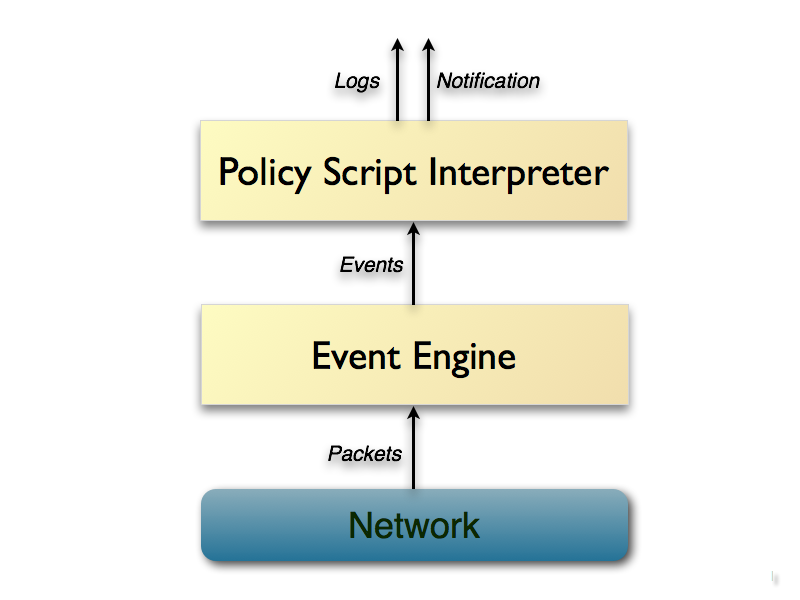
\includegraphics[width=0.5\textwidth]{imagenes/arquitectura-bro.png}
  \centering
  \caption{Arquitectura de Bro.}
\end{figure}

\subsection{Funcionalidades básicas de BRO}

La funcionalidad básica de Bro es la monitorización de la red en la que se ejecuta. 
Mientras que se encuentra en ejecución, genera registros o \textit{logs} en texto plano que se 
podrán leer usando un editor de texto. Si se analiza un archivo \textit{pcap} los \textit{logs} no cambiarán. Sin 
embargo si se analiza tráfico a tiempo real, los registros se irán actualizando a medida que pase el tiempo. 
Algunos de los \textit{logs} que se generarán son los siguientes.

\begin{itemize}
\item \textit{dpd.log}. Consiste en un resumen de los protocolos encontrados en puertos que no son estándar.
\item \textit{dns.log}. Contendrá toda la actividad correspondiente al \textit{DNS}
\item \textit{ftp.log}. Un registro de la actividad a nivel de sesión de \textit{FTP}.
\item \textit{files.log}. Un resumen con los archivos transferidos a través de una red. Incluye 
protocolos \textit{HTTP, FTP y SMTP.}
\item \textit{http.log}. Registro de toda la actividad \textit{HTTP} con sus réplicas.
\item \textit{ssl.log}. Un registro de las sesiones \textit{SSL}, incluidos los certificados que se utilizan.
\item \textit{weird.log}. En este \textit{log} se guarda la información correspondiente a actividad 
inesperada o rara a nivel de protocolo. Al analizar gran cantidad de tráfico no es muy útil, pues ocurren 
muchas cosas raras, pero a pequeña escala es bastante interesante para detectar intrusiones y demás.
\item \textit{conn.log}. Aquí se puede ver la información correspondiente a conexiones  \textit{TCP, UDP e ICMP}.
\end{itemize}

\intro Para más información sobre \textit{logs} generados por una monitorización de Bro lea \cite{brologs}.

\intro Bro dispone además de varios \textit{frameworks} que extienden su funcionalidad. Con ellos se podrá crear \textit{scripts} muy potentes. Algunas de las utilidades de estos \textit{frameworks} son las siguientes.
\begin{itemize}
\item \textit{Geolocalización}. Se podrá encontrar la localización geográfica de una IP.
\item \textit{Análisis de ficheros}. El monitor de red tiene la capacidad de trabajar con ficheros.
\item \textit{Framework de loggins}. Con este \textit{framework} se podrá extender los archivos de registro que se generan.
\item \textit{NetControl}. Este \textit{framework} permitirá tener un control muy amplio y diverso del tráfico.
\end{itemize}

\intro Para mayor conocimiento de estos \textit{frameworks} y otros lea \cite{broframeworks}.

\intro Ahora con toda esta información de los registros, el administrador del sistema podrá determinar si existen amenazas en la red o si hay algún componente defectuoso. Para ello deberá de hacer uso de los eventos con los que Bro trabaja, para sacar mayor partido a todo el trabajo que se realice sobre la red.

\subsection{Eventos y trazas}

La programación en Bro no es secuencial, no se escribe un \textit{script} y se espera que se ejecute en el orden 
en el que está escrito. La programación aquí esta orientada a eventos. Por lo tanto el orden depende de cuando 
se ejecute un determinado evento en el análisis.

\intro Un evento se da cuando Bro detecta un ``comportamiento", por ejemplo cuando detecta un paquete 
de respuesta \textit{UDP}. Si se programa para que ese evento muestre un mensaje, este se mostrará cada vez que se detecte un paquete de respuesta \textit{UDP}. Por lo tanto la programación deberá de estar pensada en función de los eventos disponibles.

\intro Dentro de cada evento se podrá hacer lo que se desee, con la información que capture ese evento. Si 
el evento captura información de una conexión \textit{TCP}, se tendrá que trabajar con esa información y las 
distintas variables globales que se hayan definido previamente.

\intro Una traza es una captura del tráfico de una red. Con casi cualquier programa de diagnóstico se puede 
realizar capturas de red. En la propia web de Bro se encuentran algunos archivos de trazas de red, en 
formato \textit{pcap}, de forma que se puedan realizar pruebas sobre ellos sin necesitar realizar una 
traza propia.

\intro En el caso de Bro se podrá generar trazas de red mediante un \textit{script} de \textit{Python}
\cite{brotrace}, el cual se puede descargar desde el repositorio de \textit{GitHub} de Bro. Con dicho script también 
se podrá trabajar sobre la traza, separando el tráfico entrante del saliente, desglosando en distintos registros 
el tipo de tráfico y demás.


\subsection{Incorporación de funcionalidades}

La incorporación de funcionalidades al monitoreo realizado por Bro es una característica muy llamativa. Gracias 
a esto se podrá realizar un análisis muy personalizado usando un \textit{script} creado por el administrador de redes. De 
esta forma podrá, por ejemplo, filtrar el tráfico de una determinada IP mientras se sigue analizando el tráfico 
de forma normal, con los registros que genera Bro de forma automática. Es una forma muy sencilla de comprobar 
si por ejemplo el servicio que administra está recibiendo demasiadas peticiones desde una misma IP. Lo cual 
sería un indicio de ataque de denegación de servicio.

\intro A la hora de incorporar funcionalidades a Bro se puede hacer todo lo que se desee. Una búsqueda rápida 
por \textit{GitHub} arrojará una gran cantidad de personas que contribuyen con una gran cantidad de nuevas 
funcionalidades \citep{gitbeacon}. Ahora lo ideal sería incorporar un módulo, de forma que si el resto 
de la comunidad lo desea pueda hacer uso de él de una forma sencilla.

\section{Emparejamiento de flujos}

La técnica de emparejamiento de flujos, fue planteada por el departamento de Teoría de la Señal, 
Telemática y Comunicaciones, \textit{TSTC}, de la Universidad de Granada, en el año 2011 \cite{presentacion} \cite{comparacion}. 
%Luego en el año 2013, el departamento realizó pruebas de la técnica de identificación en un entorno de 
%laboratorio \cite{comparacion}.

\intro En el emparejamiento de flujos, la idea de la que se parte es muy sencilla. Si dos paquetes comparten 
IP's de origen y destino, y puertos de origen y destino, se podrá decir que esos dos paquetes pertenecen a 
la misma clase. Una vez que están identificados como pertenecientes a la misma clase, lo que se debe de hacer 
es comparar los tiempos de esos paquetes, de forma que sean coherentes en el flujo. Si son muy lejanos en el 
tiempo, se podrá descartar que pertenezcan al mismo flujo. Esta idea se puede ver en \cite{comparacion} de una 
forma mucho más técnica.

\intro En el mismo artículo \cite{comparacion} se encuentra la fórmula que se sigue para el emparejamiento.

\begin{equation*}
	F(x,y)=
 	\begin{cases}
	  G(x,y), & NIP(x,y) \geq 1 \\
	  -\infty, & \text{en otro caso}
	 \end{cases}
\end{equation*}

\intro Donde tenemos que G(x,y) se corresponde con la siguiente función:

\begin{displaymath}
G(x,y) = |NIP(x,y) – 1| + 1 / (dp1(x,y) + k1) + 1 / (dp2(x,y) + k1) + 1 / (dt(x,y) + k2)
\end{displaymath}

\intro Las variables de la función son las siguientes: 

\begin{itemize}
\item \textit{x}: Primer paquete a comparar.
\item \textit{y}: Segundo paquete a comparar.
\item \textit{NIP(x,y)}: Es el número de paquetes analizados con las mismas características.
\item \textit{dp1(x,y)}: Se corresponde con los puertos de origen de los dos paquetes.
\item \textit{dp2(x,y)}: Serán los puertos de destino de los dos paquetes.
\item \textit{k1}: Es una variable definida previamente.
\item \textit{k2}: Es otra variable definida antes del comienzo del análisis. En trabajos anteriores esta variable 
y la anterior suelen estar definidas entre 1 y 10000.
\item \textit{dt}: Es la diferencia de tiempo existente entre los tiempos de inicio de los 
paquetes o \textit{timestamps}.
\end{itemize}

\intro Con esta fórmula se obtendrá como resultado un número, el cual será comparado con un umbral que se 
define previamente. Si el umbral definido es pequeño tendremos más flujos emparejados. Si el umbral es mayor 
serán menos los flujos que serán emparejados al no cumplir los requisitos.

\intro El emparejamiento de flujos, por si mismo, sólo identifica el tráfico. Por lo tanto se 
necesitará otra técnica para clasificar el tráfico.
